\begin{figure}[h]
  \centering
  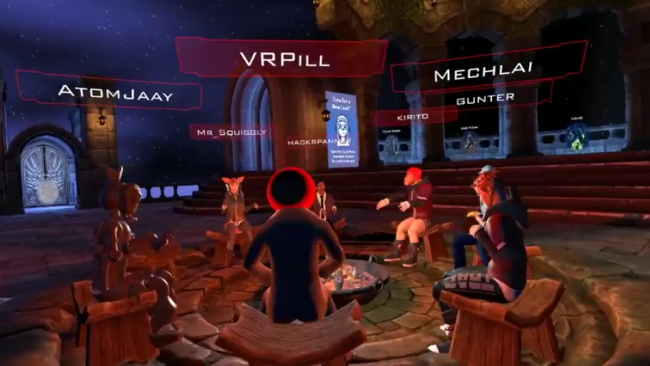
\includegraphics[width=0.8\textwidth]{images/vr_chat.png}
  \caption{In der Anwendung VR Chat können sich meherere Nutzer zum sozialen Austausch treffen. Da diese allerdings individuell navigieren, gibt es bisher keine Technik zur gemeinsamen Navigation}
  \label{fig:todo}
\end{figure}


Mit dem Verkaufsstart von Virtual Reality Headsets wie der HTC Vive oder der Oculus Rift kamen eine Vielzahl von Anwendungen und Spielen auf den Markt, von denen jedoch die überwiegende Anzahl auf einen einzelnen Nutzer ausgerichtet ist. Ausnahmen davon sind beispielsweise Apps wie VRChat\footnote{https://www.vrchat.net/}, in denen sich zahlreiche Nutzer treffen und in sozialen Austausch kommen können. Dennoch waren Forschung und Entwicklung bisher mit den Möglichkeiten und Herausforderungen dieser für einzelne Nutzer beschäftigt.

\begin{figure}[H]
	\centering
		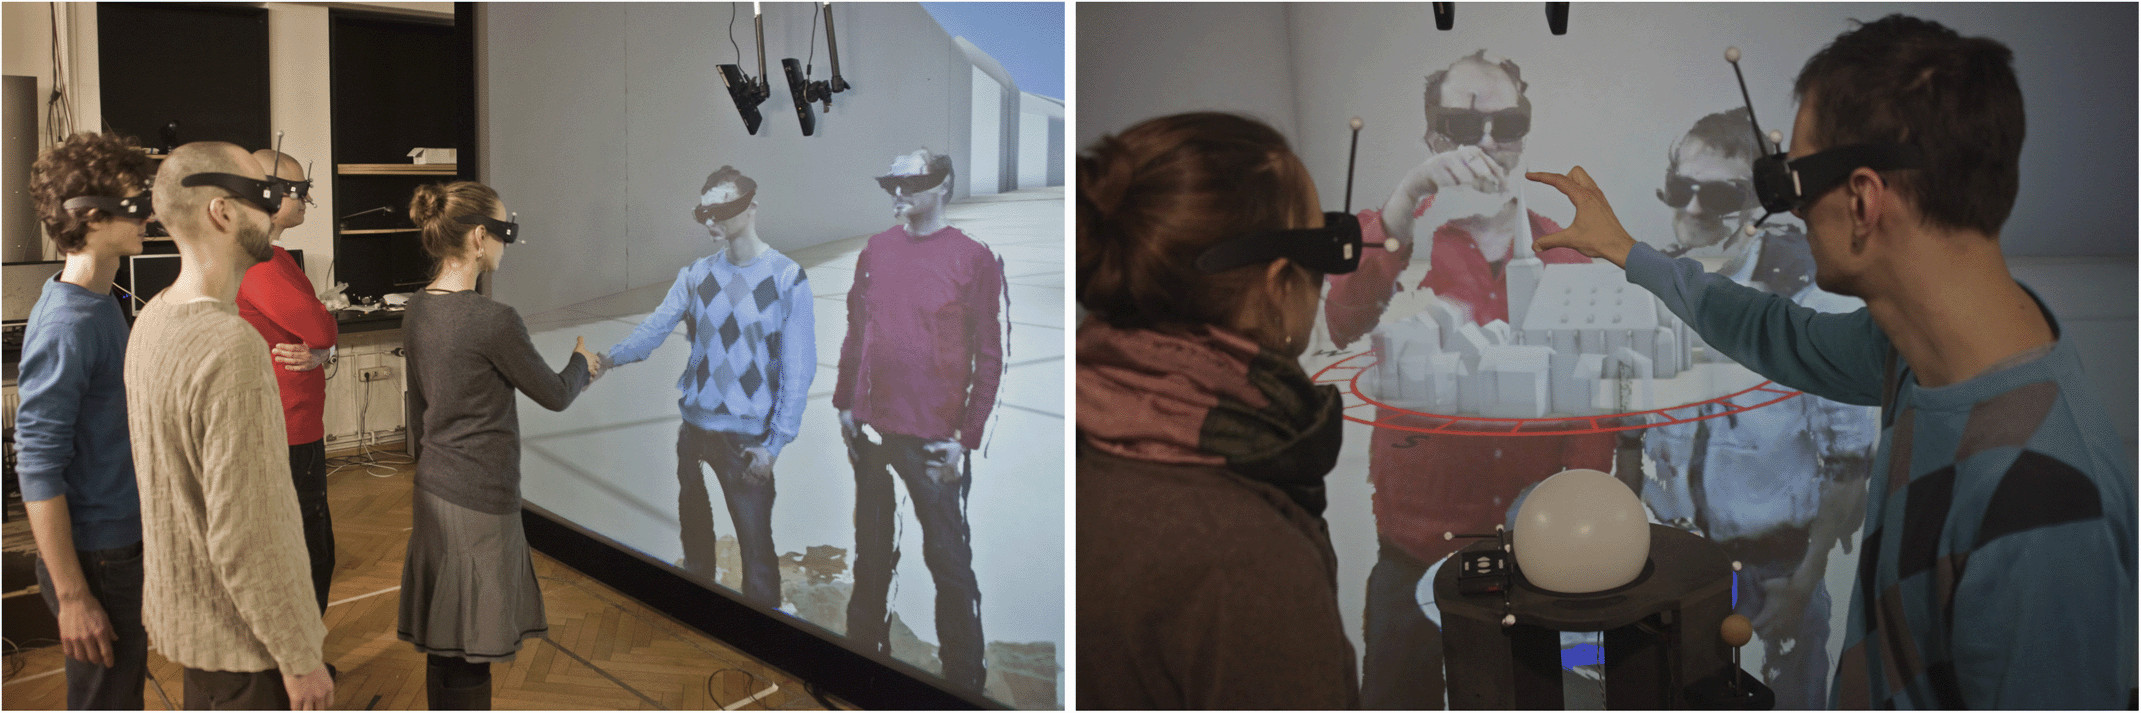
\includegraphics[width=0.8\textwidth]{images/collaborative.jpg}
	\caption{Kollaborative VR bietet die Möglichkeit sich wie auf diesem Bild virtuell zu treffen und dabei in sozialen Austausch zu treten und Umgebungen zu erkunden \cite{BeckImmersiveTelepresence}}
\end{figure}


Dabei bietet kollaborative VR ein riesiges Potential, wie bereits im einführenden Kapitel erwähnt. Gemeinsam Architekturen zu inspizieren, Datensätze zu explorieren oder Kunstwerke und Designentwürfe zu kritisieren sind Beispiele für die bereits jetzt virtuelle Realität an der Bauhaus-Universität genutzt wird. Dafür bietet unser Virtual Reality Lab neben Head Mounted Displays mehrere Mehrbenutzer oder Multi-User Leinwände, an denen bis zu sechs Personen gemeinsam eine teil-immersive virtuelle Realität bereisen können\cite{Kulik2011C1x6}. Diese bringen den Vorteil, dass die Nutzer sich in realer Form sehen können und gleichzeitig mit der virtuellen Umgebung interagieren können, wobei sie in natürlicher Form kommunizieren können.
Arbeiten zur Telepräsenz\cite{BeckImmersiveTelepresence} zeigen, dass man auch entfernte Nutzer über das Internet zuschalten kann und somit mehrere Nutzergruppen verbinden und mit lebensechten Avataren repräsentieren kann. 
Gerade im Hinblick auf die aktuellen Entwicklungen des Weltklimas und dem Anteil, den nicht zuletzt geschäftliche Flugreisen dazu beitragen, könnten gut nutzbare, kollaborative virtuelle Realitäten dazu beitragen, den Kerosinverbrauch zu minimieren, indem es für Geschäftspartner möglich ist sich in solchen Umgebungen \glqq von Angesicht zu Angesicht \grqq{} zu treffen.
Bei allen Systemen, egal ob halb oder voll immersiv, ob der Gegenüber real oder ein Avatar ist, bleibt das Problem, dass sich alle Nutzer in einem realen Raum mit realen Abmessungen befinden und sich somit zu Fuß nicht aus diesem bewegen können. Da für dieses Problem derzeit keine Lösung absehbar ist und es generell bessere Herangehensweisen gibt, als mehrere Kilometer zu Fuß zu laufen, galt und gilt es nun Navigationstechniken zu entwickeln, mit denen man die Grenzen dieses realen Raumes überwindet.

\begin{figure}[H]
	\centering
		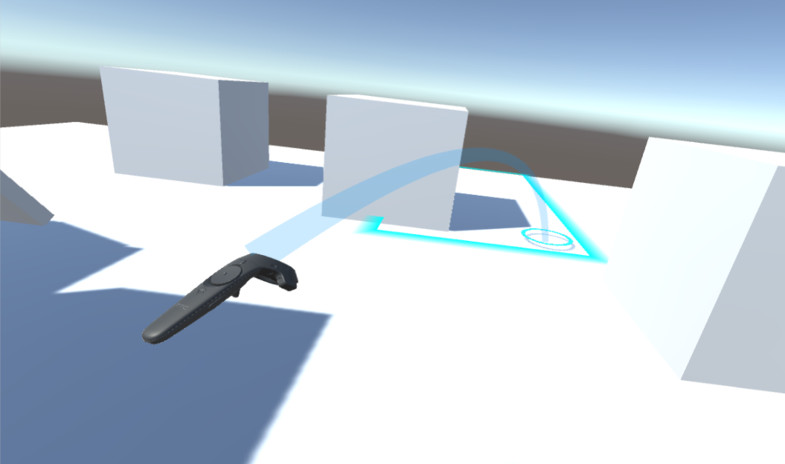
\includegraphics[width=0.8\textwidth]{images/steam_teleport.jpg}
	\caption{Für die Einzelnutzernavigation hat sich \textit{Targed-based Travel} in Form von Teleportation durchgesetzt, der im Bild sichtbar ist. Dabei bekommt der Nutzer seine künftige Position im Raum angezeigt, sowie die Grenzen seine Trackingspaces.}
\end{figure}


Während sich für kleine Distanzen und einem Nutzer der Teleport durchgesetzt hat, bei dem der Nutzer mit seinem Controller das Ziel am Ende eines Bogens auswählt (vgl. Abbildung 2.3), steigen mit zunehmender Nutzerzahl und Distanz die Möglichkeiten zur Umsetzung.
Im Falle unserer Mehrbenutzer Leinwand war das gängige Mittel die Steuerung mittels des sogenannten \textit{Spherons} (zu sehen in Abbildung 8.9), bei denen ein Steuermann die Nutzergruppe durch die Umgebung \glqq fährt\grqq{}.
Diese Technik bringt allerdings drei Nachteile mit sich. Erstens ist der Großteil der Gruppe bei der Navigation außen vor und hat als Passagier nur eingeschränktes Mitbestimmungsrecht. Dies und die damit verbundene Bewegungsparallaxe schaffen zweitens bei vielen Nutzern ein Gefühl des Unwohlseins, vor allem, wenn zur Translation im Raum auch noch eine Rotation dazukommt (vgl. dazu auch \cite{WeisskerMulti-RayReality}. Drittens eignet sich diese Vorgehensweise vor allem für kurze Distanzen und kann über größere Strecken unnötig lange dauern.
Genau an diesem Punkt soll diese Arbeit ansetzen und eine Technik finden, die die bestehende für unser Leinwandsystem ergänzt. Im Ausblick auf zukünftige Fortentwicklungen soll außerdem beschrieben werden, wie diese Technik gegebenenfalls in anderen aktuellen Systemen genutzt werden kann.